\documentclass[a4paper,10pt,titlepage]{article}

\usepackage[utf8]{inputenc}
\usepackage[T1]{fontenc}
\usepackage[danish]{babel}
\usepackage{amssymb}
\usepackage{mathtools}
\usepackage{bchart}
\usepackage{color}
\usepackage{xcolor}
\usepackage{listings}
\usepackage{float}
\usepackage{hyperref}
\hypersetup{%
    pdfborder = {0 0 0}
}

\parindent0em

\lstset{%
frame=single,
numbers=left,
numberstyle=\footnotesize,
tabsize=2,
keepspaces=true,
columns=fullflexible,
basicstyle=\ttfamily\scriptsize,
inputencoding=utf8,
extendedchars=true,
}


\begin{document}
\begin{enumerate}
\item
\textit{What is the difference between a “Data Warehouse” and a “Federated Database”?}\\

\begin{itemize}
\item
\textbf{Data Warehouse:} Is a central repository for all or significant parts of the data that an enterprise's various business systems collect. Typically, a data warehouse is housed on an enterprise mainframe server or increasingly, in the cloud. 
\item
\textbf{Federated Database:} Is a database management system, which transparently maps multiple autonomous database systems into a single federated database. This means that multiple databases appears as one database to the user.
\end{itemize}

\item
\textit{Name and describe at least four typical advantages of DBMS - based data storage over file system based data management. Give one real world example for each.}\\

\begin{enumerate}
\item
A locking mechanism for concurrent access (If users access the same item in the database there is no RW or WR errors.)
\item
The ability to swiftly recover from crashes and errors, including restartability and recoverability (If the System Crashes due to for example power failures the Logging system recovers know changes - hence reducing loss)
\item
Robust data integrity capabilities (Data is the same from all access points).
\item
Logging and auditing of activity (If changes are discarded before saving the system can re-roll.)
\end{enumerate}

\item
Design and paint an Entity Relationship (ER) diagram for a small database dedicated to store gene regulatory interactions of a bacterium. The following entities are necessary: genes (with ID and one or more (!) names), transcription factors (with ID and one name) and binding sites (with binding sequence of 10...30 bp length). Include the following relations: 
\begin{enumerate}
\item 
A transcription factor is encoded by one gene. 
\item 
A transcription factor may regulate a gene by binging to one or more binding sites.
\end{enumerate}
\begin{figure}[H]
\centering
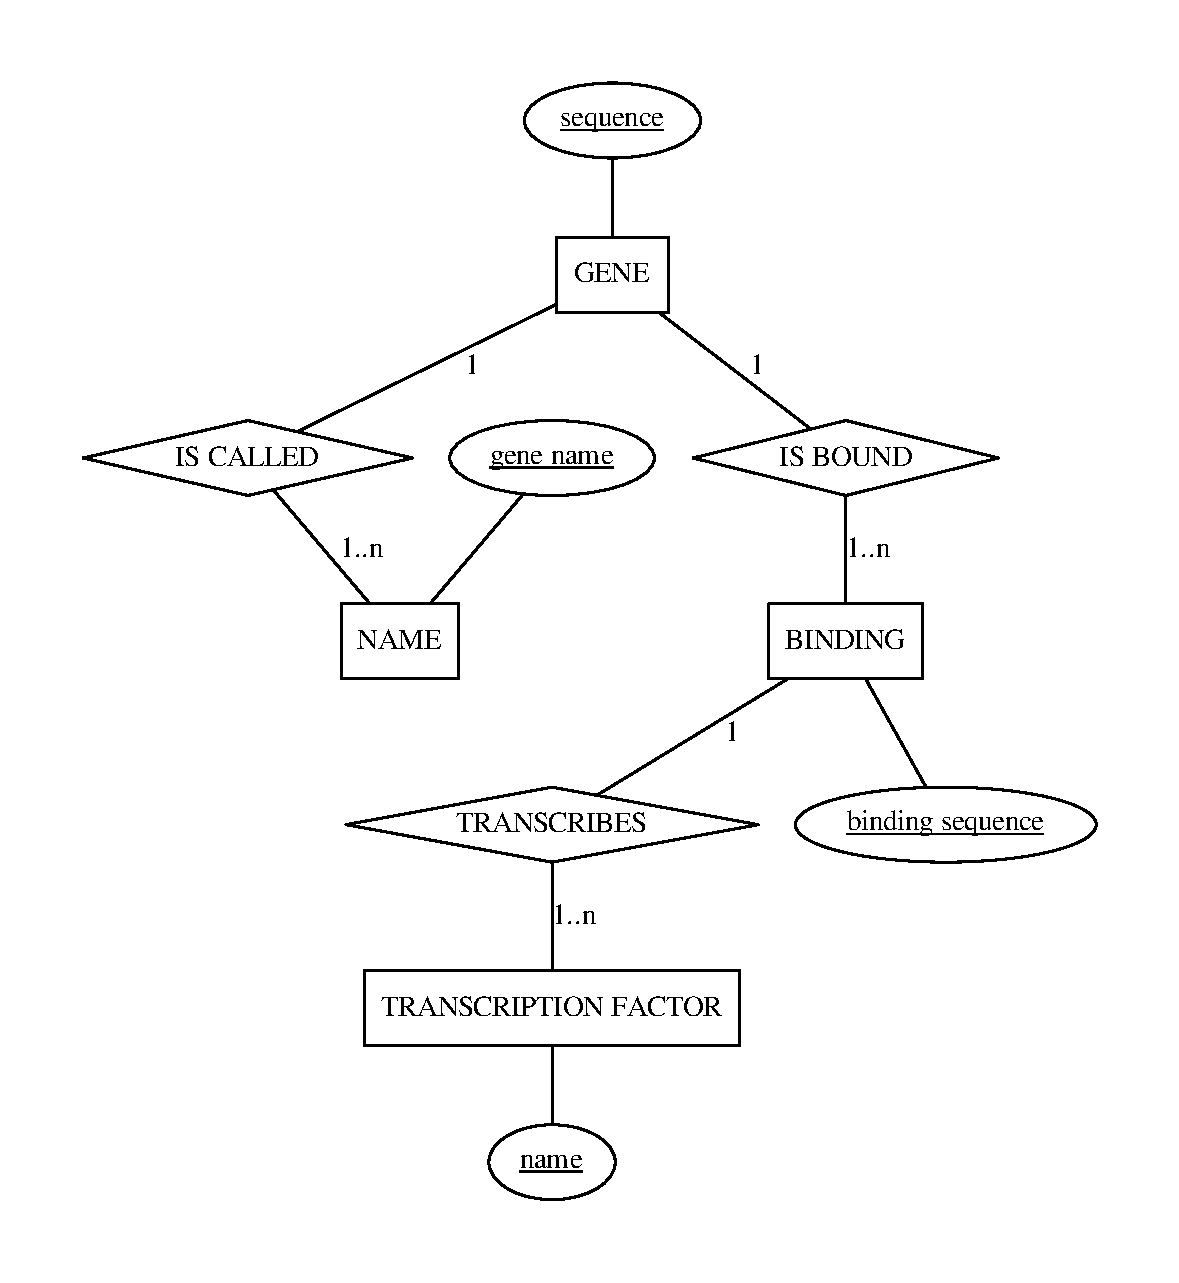
\includegraphics[scale=0.4]{graph.pdf}

\end{figure}
\item
\textit{Download and install MySQL. Design and write DDL code for MySQL that implements the in exercise 3 designed database model. Afterwards, provide DML code that fills the database with arbitrary data. Finally, give the corresponding 
SQL code for the following two queries:}
\begin{enumerate}
\item
\textit{A list of all genes that are regulated by two ore more transcription factors.}

\begin{lstlisting}
SELECT * FROM GENE WHERE 
	(
	SELECT gene_id FROM TRANSCRIPTION 
	WHERE COUNT (gene_id) > 1
	) = id;
\end{lstlisting}

\item
\textit{A list of all gene regulations. Output style: transcription factor, target gene, binding site}
\begin{lstlisting}
SELECT * FROM TRANSCRIPTION 
ORDER BY TRANSCRIPTION.name, GENE.name, BINDING_SITE.id
\end{lstlisting}
\end{enumerate}

Our DDL and DML SQL code is in the appendix of this document.

\item
\textit{Name and describe one major advantage and one major disadvantage of an ontological, generalized data structure over “standard”, explicit data structures. When would you use which approach. Explain why (give example if necessary).}\\

\begin{itemize}
\item
\textbf{Advantage:} More flexible when adding new concepts to the database.

\item
\textbf{Dis-advantage:} Hard to search due to structure. Might miss information.
\end{itemize}
Which approach?
\begin{itemize}
\item
\textbf{Ontological:} If I would need a quick overview, where I don't know if there is any structure in the data or what the structure is.
\item
\textbf{Standard:} Once a structure of the data has revealed itself.
\end{itemize}
\end{enumerate}

\appendix
\section{SQL code}

\lstset{language=SQL}
\lstinputlisting{../bioInfoDB/genes.sql}

\end{document}